\begin{figure*}[t]
\centering
\IfFileExists{figures/out/figure_s2_marcus.pdf}{%
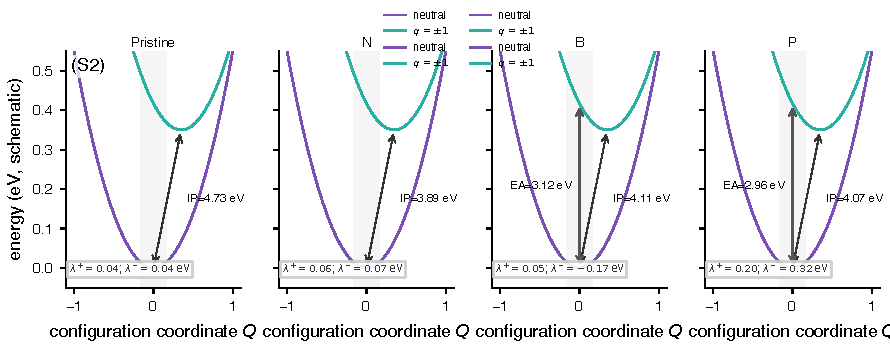
\includegraphics[width=\textwidth]{figures/out/figure_s2_marcus.pdf}}{%
\fbox{\parbox{0.85\textwidth}{\centering\vspace{2cm}\textbf{Marcus figure not found}\vspace{2cm}}}%
}
\caption{\label{fig:marcus}Marcus reorganization energies across dopants (12/12 charged-state geometry optimizations; eight vertical single-points at the neutral geometry).
Each column applies the same protocol; the slanted arrow marks adiabatic IP ($q{=}{+}1$ GEO\_OPT), teal labels give adiabatic EA where computed (B, P), and the shaded $Q{\approx}0$ band marks the neutral geometry used for vertical single-points ($\lambda^{\pm}{=}E_{\mathrm{vert}}^{\pm}-E_{\mathrm{opt}}^{\pm}$).
Pristine $\lambda^{\pm}{=}0.041$/0.042~eV; N $\lambda^{+}{=}0.058$/ $\lambda^{-}{=}0.065$~eV; B $\lambda^{+}{=}0.051$~eV; P $\lambda^{+}{=}0.200$/ $\lambda^{-}{=}0.315$~eV.
The electron-channel $\lambda^{-}$ for B is unphysical under the fixed neutral-geometry vertical protocol and is excluded (Limitations).}
\end{figure*}
